\documentclass[12pt,border=5pt]{standalone}
\usepackage[utf8]{vietnam}
\usepackage{amsmath}
\usepackage{amsfonts} 
\usepackage{amssymb}
\usepackage{tikz}
\usetikzlibrary{positioning,calc}

\begin{document}

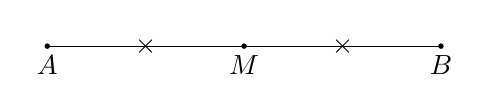
\begin{tikzpicture}
  \path
  (0, 0) coordinate (A) node[below]{$A$}
  (5, 0) coordinate (B) node[below]{$B$}
  ($(A)!.5!(B)$) coordinate (M) node[below]{$M$};

  \draw (A) -- node[midway]{$\times$} (M) -- node[midway]{$\times$} (B);

  \foreach \p in {A,M,B} \fill (\p) circle (1pt);
\end{tikzpicture}

\end{document}